% Created by tikzDevice version 0.12.3 on 2020-05-24 19:41:14
% !TEX encoding = UTF-8 Unicode
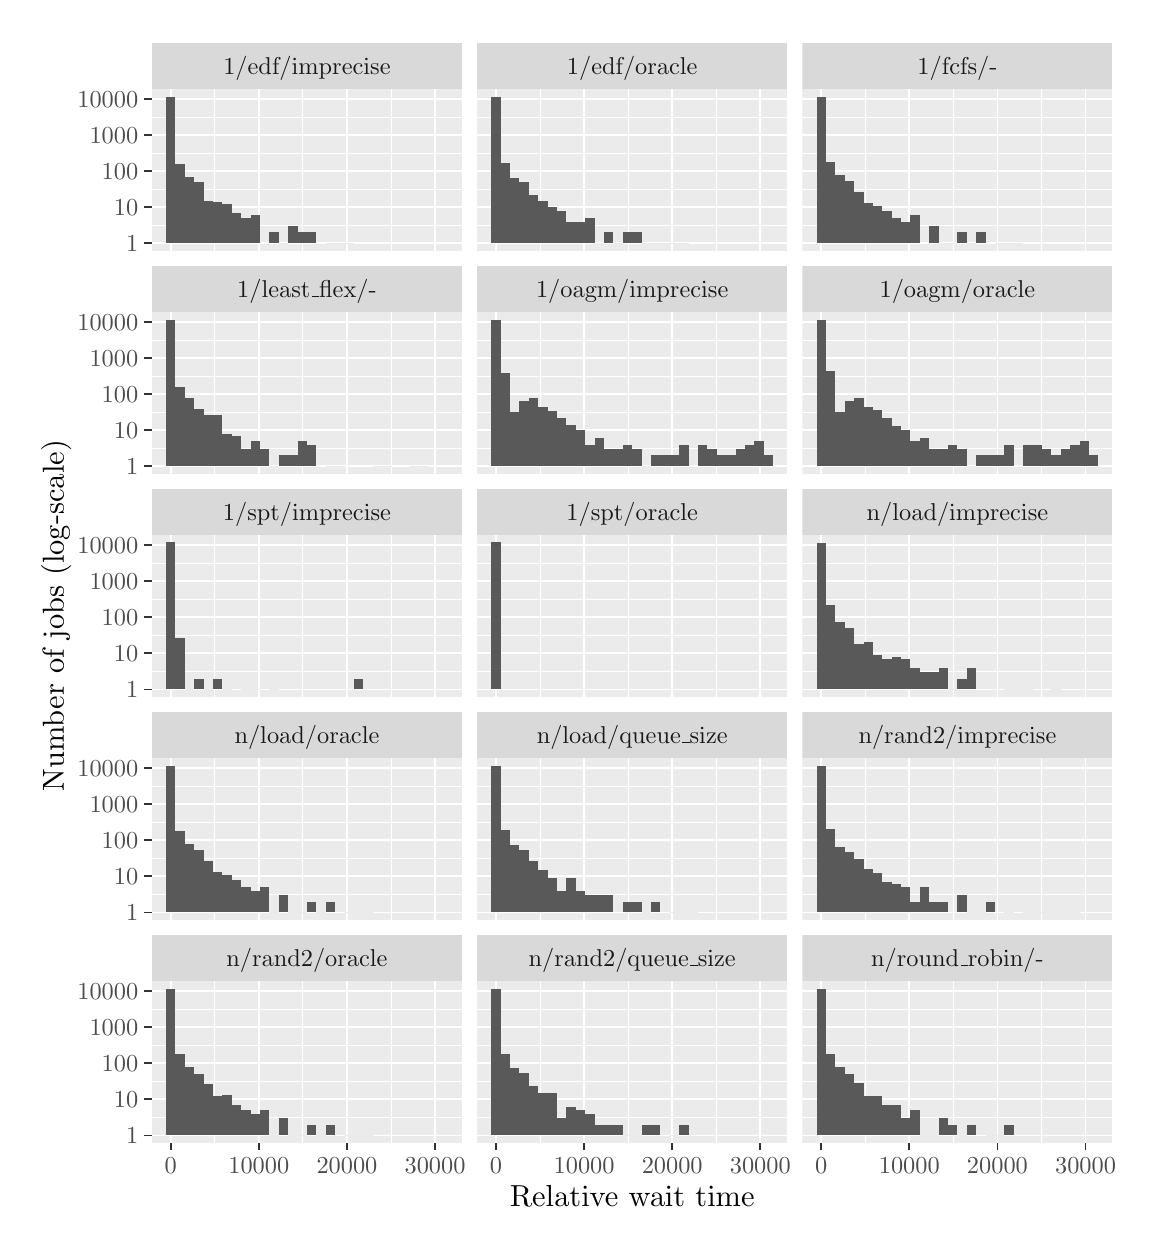
\begin{tikzpicture}[x=1pt,y=1pt]
\definecolor{fillColor}{RGB}{255,255,255}
\path[use as bounding box,fill=fillColor,fill opacity=0.00] (0,0) rectangle (397.48,433.62);
\begin{scope}
\path[clip] (  0.00,  0.00) rectangle (397.48,433.62);
\definecolor{drawColor}{RGB}{255,255,255}
\definecolor{fillColor}{RGB}{255,255,255}

\path[draw=drawColor,line width= 0.6pt,line join=round,line cap=round,fill=fillColor] (  0.00,  0.00) rectangle (397.48,433.62);
\end{scope}
\begin{scope}
\path[clip] ( 44.91,353.03) rectangle (156.93,411.55);
\definecolor{fillColor}{gray}{0.92}

\path[fill=fillColor] ( 44.91,353.03) rectangle (156.93,411.55);
\definecolor{drawColor}{RGB}{255,255,255}

\path[draw=drawColor,line width= 0.3pt,line join=round] ( 44.91,362.21) --
	(156.93,362.21);

\path[draw=drawColor,line width= 0.3pt,line join=round] ( 44.91,375.25) --
	(156.93,375.25);

\path[draw=drawColor,line width= 0.3pt,line join=round] ( 44.91,388.29) --
	(156.93,388.29);

\path[draw=drawColor,line width= 0.3pt,line join=round] ( 44.91,401.34) --
	(156.93,401.34);

\path[draw=drawColor,line width= 0.3pt,line join=round] ( 67.62,353.03) --
	( 67.62,411.55);

\path[draw=drawColor,line width= 0.3pt,line join=round] ( 99.45,353.03) --
	( 99.45,411.55);

\path[draw=drawColor,line width= 0.3pt,line join=round] (131.29,353.03) --
	(131.29,411.55);

\path[draw=drawColor,line width= 0.6pt,line join=round] ( 44.91,355.69) --
	(156.93,355.69);

\path[draw=drawColor,line width= 0.6pt,line join=round] ( 44.91,368.73) --
	(156.93,368.73);

\path[draw=drawColor,line width= 0.6pt,line join=round] ( 44.91,381.77) --
	(156.93,381.77);

\path[draw=drawColor,line width= 0.6pt,line join=round] ( 44.91,394.82) --
	(156.93,394.82);

\path[draw=drawColor,line width= 0.6pt,line join=round] ( 44.91,407.86) --
	(156.93,407.86);

\path[draw=drawColor,line width= 0.6pt,line join=round] ( 51.70,353.03) --
	( 51.70,411.55);

\path[draw=drawColor,line width= 0.6pt,line join=round] ( 83.53,353.03) --
	( 83.53,411.55);

\path[draw=drawColor,line width= 0.6pt,line join=round] (115.37,353.03) --
	(115.37,411.55);

\path[draw=drawColor,line width= 0.6pt,line join=round] (147.21,353.03) --
	(147.21,411.55);
\definecolor{fillColor}{gray}{0.35}

\path[fill=fillColor] ( 50.00,355.69) rectangle ( 53.40,408.72);

\path[fill=fillColor] ( 53.40,355.69) rectangle ( 56.79,384.44);

\path[fill=fillColor] ( 56.79,355.69) rectangle ( 60.19,379.51);

\path[fill=fillColor] ( 60.19,355.69) rectangle ( 63.58,377.73);

\path[fill=fillColor] ( 63.58,355.69) rectangle ( 66.97,371.03);

\path[fill=fillColor] ( 66.97,355.69) rectangle ( 70.37,370.64);

\path[fill=fillColor] ( 70.37,355.69) rectangle ( 73.76,369.77);

\path[fill=fillColor] ( 73.76,355.69) rectangle ( 77.16,366.71);

\path[fill=fillColor] ( 77.16,355.69) rectangle ( 80.55,364.81);

\path[fill=fillColor] ( 80.55,355.69) rectangle ( 83.95,365.84);

\path[fill=fillColor] ( 87.34,355.69) rectangle ( 90.74,359.62);

\path[fill=fillColor] ( 90.74,355.69) rectangle ( 94.13,355.69);

\path[fill=fillColor] ( 94.13,355.69) rectangle ( 97.53,361.91);

\path[fill=fillColor] ( 97.53,355.69) rectangle (100.92,359.62);

\path[fill=fillColor] (100.92,355.69) rectangle (104.32,359.62);

\path[fill=fillColor] (107.71,355.69) rectangle (111.11,355.69);

\path[fill=fillColor] (111.11,355.69) rectangle (114.50,355.69);

\path[fill=fillColor] (114.50,355.69) rectangle (117.90,355.69);
\end{scope}
\begin{scope}
\path[clip] ( 44.91,272.45) rectangle (156.93,330.96);
\definecolor{fillColor}{gray}{0.92}

\path[fill=fillColor] ( 44.91,272.45) rectangle (156.93,330.96);
\definecolor{drawColor}{RGB}{255,255,255}

\path[draw=drawColor,line width= 0.3pt,line join=round] ( 44.91,281.63) --
	(156.93,281.63);

\path[draw=drawColor,line width= 0.3pt,line join=round] ( 44.91,294.67) --
	(156.93,294.67);

\path[draw=drawColor,line width= 0.3pt,line join=round] ( 44.91,307.71) --
	(156.93,307.71);

\path[draw=drawColor,line width= 0.3pt,line join=round] ( 44.91,320.75) --
	(156.93,320.75);

\path[draw=drawColor,line width= 0.3pt,line join=round] ( 67.62,272.45) --
	( 67.62,330.96);

\path[draw=drawColor,line width= 0.3pt,line join=round] ( 99.45,272.45) --
	( 99.45,330.96);

\path[draw=drawColor,line width= 0.3pt,line join=round] (131.29,272.45) --
	(131.29,330.96);

\path[draw=drawColor,line width= 0.6pt,line join=round] ( 44.91,275.11) --
	(156.93,275.11);

\path[draw=drawColor,line width= 0.6pt,line join=round] ( 44.91,288.15) --
	(156.93,288.15);

\path[draw=drawColor,line width= 0.6pt,line join=round] ( 44.91,301.19) --
	(156.93,301.19);

\path[draw=drawColor,line width= 0.6pt,line join=round] ( 44.91,314.23) --
	(156.93,314.23);

\path[draw=drawColor,line width= 0.6pt,line join=round] ( 44.91,327.27) --
	(156.93,327.27);

\path[draw=drawColor,line width= 0.6pt,line join=round] ( 51.70,272.45) --
	( 51.70,330.96);

\path[draw=drawColor,line width= 0.6pt,line join=round] ( 83.53,272.45) --
	( 83.53,330.96);

\path[draw=drawColor,line width= 0.6pt,line join=round] (115.37,272.45) --
	(115.37,330.96);

\path[draw=drawColor,line width= 0.6pt,line join=round] (147.21,272.45) --
	(147.21,330.96);
\definecolor{fillColor}{gray}{0.35}

\path[fill=fillColor] ( 50.00,275.11) rectangle ( 53.40,328.12);

\path[fill=fillColor] ( 53.40,275.11) rectangle ( 56.79,303.95);

\path[fill=fillColor] ( 56.79,275.11) rectangle ( 60.19,299.78);

\path[fill=fillColor] ( 60.19,275.11) rectangle ( 63.58,295.71);

\path[fill=fillColor] ( 63.58,275.11) rectangle ( 66.97,293.77);

\path[fill=fillColor] ( 66.97,275.11) rectangle ( 70.37,293.77);

\path[fill=fillColor] ( 70.37,275.11) rectangle ( 73.76,286.88);

\path[fill=fillColor] ( 73.76,275.11) rectangle ( 77.16,286.13);

\path[fill=fillColor] ( 77.16,275.11) rectangle ( 80.55,281.33);

\path[fill=fillColor] ( 80.55,275.11) rectangle ( 83.95,284.22);

\path[fill=fillColor] ( 83.95,275.11) rectangle ( 87.34,281.33);

\path[fill=fillColor] ( 87.34,275.11) rectangle ( 90.74,275.11);

\path[fill=fillColor] ( 90.74,275.11) rectangle ( 94.13,279.03);

\path[fill=fillColor] ( 94.13,275.11) rectangle ( 97.53,279.03);

\path[fill=fillColor] ( 97.53,275.11) rectangle (100.92,284.22);

\path[fill=fillColor] (100.92,275.11) rectangle (104.32,282.96);

\path[fill=fillColor] (107.71,275.11) rectangle (111.11,275.11);

\path[fill=fillColor] (111.11,275.11) rectangle (114.50,275.11);

\path[fill=fillColor] (124.68,275.11) rectangle (128.08,275.11);

\path[fill=fillColor] (128.08,275.11) rectangle (131.47,275.11);

\path[fill=fillColor] (138.26,275.11) rectangle (141.66,275.11);

\path[fill=fillColor] (141.66,275.11) rectangle (145.05,275.11);
\end{scope}
\begin{scope}
\path[clip] ( 44.91,191.86) rectangle (156.93,250.37);
\definecolor{fillColor}{gray}{0.92}

\path[fill=fillColor] ( 44.91,191.86) rectangle (156.93,250.37);
\definecolor{drawColor}{RGB}{255,255,255}

\path[draw=drawColor,line width= 0.3pt,line join=round] ( 44.91,201.04) --
	(156.93,201.04);

\path[draw=drawColor,line width= 0.3pt,line join=round] ( 44.91,214.08) --
	(156.93,214.08);

\path[draw=drawColor,line width= 0.3pt,line join=round] ( 44.91,227.12) --
	(156.93,227.12);

\path[draw=drawColor,line width= 0.3pt,line join=round] ( 44.91,240.16) --
	(156.93,240.16);

\path[draw=drawColor,line width= 0.3pt,line join=round] ( 67.62,191.86) --
	( 67.62,250.37);

\path[draw=drawColor,line width= 0.3pt,line join=round] ( 99.45,191.86) --
	( 99.45,250.37);

\path[draw=drawColor,line width= 0.3pt,line join=round] (131.29,191.86) --
	(131.29,250.37);

\path[draw=drawColor,line width= 0.6pt,line join=round] ( 44.91,194.52) --
	(156.93,194.52);

\path[draw=drawColor,line width= 0.6pt,line join=round] ( 44.91,207.56) --
	(156.93,207.56);

\path[draw=drawColor,line width= 0.6pt,line join=round] ( 44.91,220.60) --
	(156.93,220.60);

\path[draw=drawColor,line width= 0.6pt,line join=round] ( 44.91,233.64) --
	(156.93,233.64);

\path[draw=drawColor,line width= 0.6pt,line join=round] ( 44.91,246.68) --
	(156.93,246.68);

\path[draw=drawColor,line width= 0.6pt,line join=round] ( 51.70,191.86) --
	( 51.70,250.37);

\path[draw=drawColor,line width= 0.6pt,line join=round] ( 83.53,191.86) --
	( 83.53,250.37);

\path[draw=drawColor,line width= 0.6pt,line join=round] (115.37,191.86) --
	(115.37,250.37);

\path[draw=drawColor,line width= 0.6pt,line join=round] (147.21,191.86) --
	(147.21,250.37);
\definecolor{fillColor}{gray}{0.35}

\path[fill=fillColor] ( 50.00,194.52) rectangle ( 53.40,247.70);

\path[fill=fillColor] ( 53.40,194.52) rectangle ( 56.79,213.19);

\path[fill=fillColor] ( 56.79,194.52) rectangle ( 60.19,194.52);

\path[fill=fillColor] ( 60.19,194.52) rectangle ( 63.58,198.44);

\path[fill=fillColor] ( 63.58,194.52) rectangle ( 66.97,194.52);

\path[fill=fillColor] ( 66.97,194.52) rectangle ( 70.37,198.44);

\path[fill=fillColor] ( 70.37,194.52) rectangle ( 73.76,194.52);

\path[fill=fillColor] ( 77.16,194.52) rectangle ( 80.55,194.52);

\path[fill=fillColor] ( 80.55,194.52) rectangle ( 83.95,194.52);

\path[fill=fillColor] ( 87.34,194.52) rectangle ( 90.74,194.52);

\path[fill=fillColor] (117.90,194.52) rectangle (121.29,198.44);
\end{scope}
\begin{scope}
\path[clip] ( 44.91,111.27) rectangle (156.93,169.79);
\definecolor{fillColor}{gray}{0.92}

\path[fill=fillColor] ( 44.91,111.27) rectangle (156.93,169.79);
\definecolor{drawColor}{RGB}{255,255,255}

\path[draw=drawColor,line width= 0.3pt,line join=round] ( 44.91,120.45) --
	(156.93,120.45);

\path[draw=drawColor,line width= 0.3pt,line join=round] ( 44.91,133.49) --
	(156.93,133.49);

\path[draw=drawColor,line width= 0.3pt,line join=round] ( 44.91,146.53) --
	(156.93,146.53);

\path[draw=drawColor,line width= 0.3pt,line join=round] ( 44.91,159.58) --
	(156.93,159.58);

\path[draw=drawColor,line width= 0.3pt,line join=round] ( 67.62,111.27) --
	( 67.62,169.79);

\path[draw=drawColor,line width= 0.3pt,line join=round] ( 99.45,111.27) --
	( 99.45,169.79);

\path[draw=drawColor,line width= 0.3pt,line join=round] (131.29,111.27) --
	(131.29,169.79);

\path[draw=drawColor,line width= 0.6pt,line join=round] ( 44.91,113.93) --
	(156.93,113.93);

\path[draw=drawColor,line width= 0.6pt,line join=round] ( 44.91,126.97) --
	(156.93,126.97);

\path[draw=drawColor,line width= 0.6pt,line join=round] ( 44.91,140.01) --
	(156.93,140.01);

\path[draw=drawColor,line width= 0.6pt,line join=round] ( 44.91,153.05) --
	(156.93,153.05);

\path[draw=drawColor,line width= 0.6pt,line join=round] ( 44.91,166.10) --
	(156.93,166.10);

\path[draw=drawColor,line width= 0.6pt,line join=round] ( 51.70,111.27) --
	( 51.70,169.79);

\path[draw=drawColor,line width= 0.6pt,line join=round] ( 83.53,111.27) --
	( 83.53,169.79);

\path[draw=drawColor,line width= 0.6pt,line join=round] (115.37,111.27) --
	(115.37,169.79);

\path[draw=drawColor,line width= 0.6pt,line join=round] (147.21,111.27) --
	(147.21,169.79);
\definecolor{fillColor}{gray}{0.35}

\path[fill=fillColor] ( 50.00,113.93) rectangle ( 53.40,166.94);

\path[fill=fillColor] ( 53.40,113.93) rectangle ( 56.79,143.34);

\path[fill=fillColor] ( 56.79,113.93) rectangle ( 60.19,138.53);

\path[fill=fillColor] ( 60.19,113.93) rectangle ( 63.58,136.31);

\path[fill=fillColor] ( 63.58,113.93) rectangle ( 66.97,132.38);

\path[fill=fillColor] ( 66.97,113.93) rectangle ( 70.37,128.46);

\path[fill=fillColor] ( 70.37,113.93) rectangle ( 73.76,127.51);

\path[fill=fillColor] ( 73.76,113.93) rectangle ( 77.16,125.71);

\path[fill=fillColor] ( 77.16,113.93) rectangle ( 80.55,123.05);

\path[fill=fillColor] ( 80.55,113.93) rectangle ( 83.95,121.78);

\path[fill=fillColor] ( 83.95,113.93) rectangle ( 87.34,123.05);

\path[fill=fillColor] ( 87.34,113.93) rectangle ( 90.74,113.93);

\path[fill=fillColor] ( 90.74,113.93) rectangle ( 94.13,120.15);

\path[fill=fillColor] ( 94.13,113.93) rectangle ( 97.53,113.93);

\path[fill=fillColor] ( 97.53,113.93) rectangle (100.92,113.93);

\path[fill=fillColor] (100.92,113.93) rectangle (104.32,117.86);

\path[fill=fillColor] (104.32,113.93) rectangle (107.71,113.93);

\path[fill=fillColor] (107.71,113.93) rectangle (111.11,117.86);

\path[fill=fillColor] (114.50,113.93) rectangle (117.90,113.93);

\path[fill=fillColor] (117.90,113.93) rectangle (121.29,113.93);

\path[fill=fillColor] (121.29,113.93) rectangle (124.68,113.93);
\end{scope}
\begin{scope}
\path[clip] ( 44.91, 30.69) rectangle (156.93, 89.20);
\definecolor{fillColor}{gray}{0.92}

\path[fill=fillColor] ( 44.91, 30.69) rectangle (156.93, 89.20);
\definecolor{drawColor}{RGB}{255,255,255}

\path[draw=drawColor,line width= 0.3pt,line join=round] ( 44.91, 39.87) --
	(156.93, 39.87);

\path[draw=drawColor,line width= 0.3pt,line join=round] ( 44.91, 52.91) --
	(156.93, 52.91);

\path[draw=drawColor,line width= 0.3pt,line join=round] ( 44.91, 65.95) --
	(156.93, 65.95);

\path[draw=drawColor,line width= 0.3pt,line join=round] ( 44.91, 78.99) --
	(156.93, 78.99);

\path[draw=drawColor,line width= 0.3pt,line join=round] ( 67.62, 30.69) --
	( 67.62, 89.20);

\path[draw=drawColor,line width= 0.3pt,line join=round] ( 99.45, 30.69) --
	( 99.45, 89.20);

\path[draw=drawColor,line width= 0.3pt,line join=round] (131.29, 30.69) --
	(131.29, 89.20);

\path[draw=drawColor,line width= 0.6pt,line join=round] ( 44.91, 33.35) --
	(156.93, 33.35);

\path[draw=drawColor,line width= 0.6pt,line join=round] ( 44.91, 46.39) --
	(156.93, 46.39);

\path[draw=drawColor,line width= 0.6pt,line join=round] ( 44.91, 59.43) --
	(156.93, 59.43);

\path[draw=drawColor,line width= 0.6pt,line join=round] ( 44.91, 72.47) --
	(156.93, 72.47);

\path[draw=drawColor,line width= 0.6pt,line join=round] ( 44.91, 85.51) --
	(156.93, 85.51);

\path[draw=drawColor,line width= 0.6pt,line join=round] ( 51.70, 30.69) --
	( 51.70, 89.20);

\path[draw=drawColor,line width= 0.6pt,line join=round] ( 83.53, 30.69) --
	( 83.53, 89.20);

\path[draw=drawColor,line width= 0.6pt,line join=round] (115.37, 30.69) --
	(115.37, 89.20);

\path[draw=drawColor,line width= 0.6pt,line join=round] (147.21, 30.69) --
	(147.21, 89.20);
\definecolor{fillColor}{gray}{0.35}

\path[fill=fillColor] ( 50.00, 33.35) rectangle ( 53.40, 86.35);

\path[fill=fillColor] ( 53.40, 33.35) rectangle ( 56.79, 62.66);

\path[fill=fillColor] ( 56.79, 33.35) rectangle ( 60.19, 58.02);

\path[fill=fillColor] ( 60.19, 33.35) rectangle ( 63.58, 55.61);

\path[fill=fillColor] ( 63.58, 33.35) rectangle ( 66.97, 51.80);

\path[fill=fillColor] ( 66.97, 33.35) rectangle ( 70.37, 47.42);

\path[fill=fillColor] ( 70.37, 33.35) rectangle ( 73.76, 47.87);

\path[fill=fillColor] ( 73.76, 33.35) rectangle ( 77.16, 44.37);

\path[fill=fillColor] ( 77.16, 33.35) rectangle ( 80.55, 42.46);

\path[fill=fillColor] ( 80.55, 33.35) rectangle ( 83.95, 41.20);

\path[fill=fillColor] ( 83.95, 33.35) rectangle ( 87.34, 42.46);

\path[fill=fillColor] ( 87.34, 33.35) rectangle ( 90.74, 33.35);

\path[fill=fillColor] ( 90.74, 33.35) rectangle ( 94.13, 39.57);

\path[fill=fillColor] ( 94.13, 33.35) rectangle ( 97.53, 33.35);

\path[fill=fillColor] ( 97.53, 33.35) rectangle (100.92, 33.35);

\path[fill=fillColor] (100.92, 33.35) rectangle (104.32, 37.27);

\path[fill=fillColor] (104.32, 33.35) rectangle (107.71, 33.35);

\path[fill=fillColor] (107.71, 33.35) rectangle (111.11, 37.27);

\path[fill=fillColor] (114.50, 33.35) rectangle (117.90, 33.35);

\path[fill=fillColor] (117.90, 33.35) rectangle (121.29, 33.35);

\path[fill=fillColor] (121.29, 33.35) rectangle (124.68, 33.35);
\end{scope}
\begin{scope}
\path[clip] (162.43,353.03) rectangle (274.46,411.55);
\definecolor{fillColor}{gray}{0.92}

\path[fill=fillColor] (162.43,353.03) rectangle (274.46,411.55);
\definecolor{drawColor}{RGB}{255,255,255}

\path[draw=drawColor,line width= 0.3pt,line join=round] (162.43,362.21) --
	(274.46,362.21);

\path[draw=drawColor,line width= 0.3pt,line join=round] (162.43,375.25) --
	(274.46,375.25);

\path[draw=drawColor,line width= 0.3pt,line join=round] (162.43,388.29) --
	(274.46,388.29);

\path[draw=drawColor,line width= 0.3pt,line join=round] (162.43,401.34) --
	(274.46,401.34);

\path[draw=drawColor,line width= 0.3pt,line join=round] (185.14,353.03) --
	(185.14,411.55);

\path[draw=drawColor,line width= 0.3pt,line join=round] (216.98,353.03) --
	(216.98,411.55);

\path[draw=drawColor,line width= 0.3pt,line join=round] (248.81,353.03) --
	(248.81,411.55);

\path[draw=drawColor,line width= 0.6pt,line join=round] (162.43,355.69) --
	(274.46,355.69);

\path[draw=drawColor,line width= 0.6pt,line join=round] (162.43,368.73) --
	(274.46,368.73);

\path[draw=drawColor,line width= 0.6pt,line join=round] (162.43,381.77) --
	(274.46,381.77);

\path[draw=drawColor,line width= 0.6pt,line join=round] (162.43,394.82) --
	(274.46,394.82);

\path[draw=drawColor,line width= 0.6pt,line join=round] (162.43,407.86) --
	(274.46,407.86);

\path[draw=drawColor,line width= 0.6pt,line join=round] (169.22,353.03) --
	(169.22,411.55);

\path[draw=drawColor,line width= 0.6pt,line join=round] (201.06,353.03) --
	(201.06,411.55);

\path[draw=drawColor,line width= 0.6pt,line join=round] (232.90,353.03) --
	(232.90,411.55);

\path[draw=drawColor,line width= 0.6pt,line join=round] (264.73,353.03) --
	(264.73,411.55);
\definecolor{fillColor}{gray}{0.35}

\path[fill=fillColor] (167.53,355.69) rectangle (170.92,408.71);

\path[fill=fillColor] (170.92,355.69) rectangle (174.32,384.71);

\path[fill=fillColor] (174.32,355.69) rectangle (177.71,379.42);

\path[fill=fillColor] (177.71,355.69) rectangle (181.11,377.96);

\path[fill=fillColor] (181.11,355.69) rectangle (184.50,373.20);

\path[fill=fillColor] (184.50,355.69) rectangle (187.89,371.03);

\path[fill=fillColor] (187.89,355.69) rectangle (191.29,368.73);

\path[fill=fillColor] (191.29,355.69) rectangle (194.68,367.47);

\path[fill=fillColor] (194.68,355.69) rectangle (198.08,363.54);

\path[fill=fillColor] (198.08,355.69) rectangle (201.47,363.54);

\path[fill=fillColor] (201.47,355.69) rectangle (204.87,364.81);

\path[fill=fillColor] (204.87,355.69) rectangle (208.26,355.69);

\path[fill=fillColor] (208.26,355.69) rectangle (211.66,359.62);

\path[fill=fillColor] (211.66,355.69) rectangle (215.05,355.69);

\path[fill=fillColor] (215.05,355.69) rectangle (218.45,359.62);

\path[fill=fillColor] (218.45,355.69) rectangle (221.84,359.62);

\path[fill=fillColor] (221.84,355.69) rectangle (225.24,355.69);

\path[fill=fillColor] (225.24,355.69) rectangle (228.63,355.69);

\path[fill=fillColor] (228.63,355.69) rectangle (232.03,355.69);

\path[fill=fillColor] (232.03,355.69) rectangle (235.42,355.69);

\path[fill=fillColor] (235.42,355.69) rectangle (238.82,355.69);
\end{scope}
\begin{scope}
\path[clip] (162.43,272.45) rectangle (274.46,330.96);
\definecolor{fillColor}{gray}{0.92}

\path[fill=fillColor] (162.43,272.45) rectangle (274.46,330.96);
\definecolor{drawColor}{RGB}{255,255,255}

\path[draw=drawColor,line width= 0.3pt,line join=round] (162.43,281.63) --
	(274.46,281.63);

\path[draw=drawColor,line width= 0.3pt,line join=round] (162.43,294.67) --
	(274.46,294.67);

\path[draw=drawColor,line width= 0.3pt,line join=round] (162.43,307.71) --
	(274.46,307.71);

\path[draw=drawColor,line width= 0.3pt,line join=round] (162.43,320.75) --
	(274.46,320.75);

\path[draw=drawColor,line width= 0.3pt,line join=round] (185.14,272.45) --
	(185.14,330.96);

\path[draw=drawColor,line width= 0.3pt,line join=round] (216.98,272.45) --
	(216.98,330.96);

\path[draw=drawColor,line width= 0.3pt,line join=round] (248.81,272.45) --
	(248.81,330.96);

\path[draw=drawColor,line width= 0.6pt,line join=round] (162.43,275.11) --
	(274.46,275.11);

\path[draw=drawColor,line width= 0.6pt,line join=round] (162.43,288.15) --
	(274.46,288.15);

\path[draw=drawColor,line width= 0.6pt,line join=round] (162.43,301.19) --
	(274.46,301.19);

\path[draw=drawColor,line width= 0.6pt,line join=round] (162.43,314.23) --
	(274.46,314.23);

\path[draw=drawColor,line width= 0.6pt,line join=round] (162.43,327.27) --
	(274.46,327.27);

\path[draw=drawColor,line width= 0.6pt,line join=round] (169.22,272.45) --
	(169.22,330.96);

\path[draw=drawColor,line width= 0.6pt,line join=round] (201.06,272.45) --
	(201.06,330.96);

\path[draw=drawColor,line width= 0.6pt,line join=round] (232.90,272.45) --
	(232.90,330.96);

\path[draw=drawColor,line width= 0.6pt,line join=round] (264.73,272.45) --
	(264.73,330.96);
\definecolor{fillColor}{gray}{0.35}

\path[fill=fillColor] (167.53,275.11) rectangle (170.92,327.94);

\path[fill=fillColor] (170.92,275.11) rectangle (174.32,308.98);

\path[fill=fillColor] (174.32,275.11) rectangle (177.71,294.73);

\path[fill=fillColor] (177.71,275.11) rectangle (181.11,298.66);

\path[fill=fillColor] (181.11,275.11) rectangle (184.50,299.71);

\path[fill=fillColor] (184.50,275.11) rectangle (187.89,296.41);

\path[fill=fillColor] (187.89,275.11) rectangle (191.29,295.24);

\path[fill=fillColor] (191.29,275.11) rectangle (194.68,292.61);

\path[fill=fillColor] (194.68,275.11) rectangle (198.08,290.05);

\path[fill=fillColor] (198.08,275.11) rectangle (201.47,288.15);

\path[fill=fillColor] (201.47,275.11) rectangle (204.87,282.96);

\path[fill=fillColor] (204.87,275.11) rectangle (208.26,285.25);

\path[fill=fillColor] (208.26,275.11) rectangle (211.66,281.33);

\path[fill=fillColor] (211.66,275.11) rectangle (215.05,281.33);

\path[fill=fillColor] (215.05,275.11) rectangle (218.45,282.96);

\path[fill=fillColor] (218.45,275.11) rectangle (221.84,281.33);

\path[fill=fillColor] (221.84,275.11) rectangle (225.24,275.11);

\path[fill=fillColor] (225.24,275.11) rectangle (228.63,279.03);

\path[fill=fillColor] (228.63,275.11) rectangle (232.03,279.03);

\path[fill=fillColor] (232.03,275.11) rectangle (235.42,279.03);

\path[fill=fillColor] (235.42,275.11) rectangle (238.82,282.96);

\path[fill=fillColor] (242.21,275.11) rectangle (245.60,282.96);

\path[fill=fillColor] (245.60,275.11) rectangle (249.00,281.33);

\path[fill=fillColor] (249.00,275.11) rectangle (252.39,279.03);

\path[fill=fillColor] (252.39,275.11) rectangle (255.79,279.03);

\path[fill=fillColor] (255.79,275.11) rectangle (259.18,281.33);

\path[fill=fillColor] (259.18,275.11) rectangle (262.58,282.96);

\path[fill=fillColor] (262.58,275.11) rectangle (265.97,284.22);

\path[fill=fillColor] (265.97,275.11) rectangle (269.37,279.03);
\end{scope}
\begin{scope}
\path[clip] (162.43,191.86) rectangle (274.46,250.37);
\definecolor{fillColor}{gray}{0.92}

\path[fill=fillColor] (162.43,191.86) rectangle (274.46,250.37);
\definecolor{drawColor}{RGB}{255,255,255}

\path[draw=drawColor,line width= 0.3pt,line join=round] (162.43,201.04) --
	(274.46,201.04);

\path[draw=drawColor,line width= 0.3pt,line join=round] (162.43,214.08) --
	(274.46,214.08);

\path[draw=drawColor,line width= 0.3pt,line join=round] (162.43,227.12) --
	(274.46,227.12);

\path[draw=drawColor,line width= 0.3pt,line join=round] (162.43,240.16) --
	(274.46,240.16);

\path[draw=drawColor,line width= 0.3pt,line join=round] (185.14,191.86) --
	(185.14,250.37);

\path[draw=drawColor,line width= 0.3pt,line join=round] (216.98,191.86) --
	(216.98,250.37);

\path[draw=drawColor,line width= 0.3pt,line join=round] (248.81,191.86) --
	(248.81,250.37);

\path[draw=drawColor,line width= 0.6pt,line join=round] (162.43,194.52) --
	(274.46,194.52);

\path[draw=drawColor,line width= 0.6pt,line join=round] (162.43,207.56) --
	(274.46,207.56);

\path[draw=drawColor,line width= 0.6pt,line join=round] (162.43,220.60) --
	(274.46,220.60);

\path[draw=drawColor,line width= 0.6pt,line join=round] (162.43,233.64) --
	(274.46,233.64);

\path[draw=drawColor,line width= 0.6pt,line join=round] (162.43,246.68) --
	(274.46,246.68);

\path[draw=drawColor,line width= 0.6pt,line join=round] (169.22,191.86) --
	(169.22,250.37);

\path[draw=drawColor,line width= 0.6pt,line join=round] (201.06,191.86) --
	(201.06,250.37);

\path[draw=drawColor,line width= 0.6pt,line join=round] (232.90,191.86) --
	(232.90,250.37);

\path[draw=drawColor,line width= 0.6pt,line join=round] (264.73,191.86) --
	(264.73,250.37);
\definecolor{fillColor}{gray}{0.35}

\path[fill=fillColor] (167.53,194.52) rectangle (170.92,247.72);
\end{scope}
\begin{scope}
\path[clip] (162.43,111.27) rectangle (274.46,169.79);
\definecolor{fillColor}{gray}{0.92}

\path[fill=fillColor] (162.43,111.27) rectangle (274.46,169.79);
\definecolor{drawColor}{RGB}{255,255,255}

\path[draw=drawColor,line width= 0.3pt,line join=round] (162.43,120.45) --
	(274.46,120.45);

\path[draw=drawColor,line width= 0.3pt,line join=round] (162.43,133.49) --
	(274.46,133.49);

\path[draw=drawColor,line width= 0.3pt,line join=round] (162.43,146.53) --
	(274.46,146.53);

\path[draw=drawColor,line width= 0.3pt,line join=round] (162.43,159.58) --
	(274.46,159.58);

\path[draw=drawColor,line width= 0.3pt,line join=round] (185.14,111.27) --
	(185.14,169.79);

\path[draw=drawColor,line width= 0.3pt,line join=round] (216.98,111.27) --
	(216.98,169.79);

\path[draw=drawColor,line width= 0.3pt,line join=round] (248.81,111.27) --
	(248.81,169.79);

\path[draw=drawColor,line width= 0.6pt,line join=round] (162.43,113.93) --
	(274.46,113.93);

\path[draw=drawColor,line width= 0.6pt,line join=round] (162.43,126.97) --
	(274.46,126.97);

\path[draw=drawColor,line width= 0.6pt,line join=round] (162.43,140.01) --
	(274.46,140.01);

\path[draw=drawColor,line width= 0.6pt,line join=round] (162.43,153.05) --
	(274.46,153.05);

\path[draw=drawColor,line width= 0.6pt,line join=round] (162.43,166.10) --
	(274.46,166.10);

\path[draw=drawColor,line width= 0.6pt,line join=round] (169.22,111.27) --
	(169.22,169.79);

\path[draw=drawColor,line width= 0.6pt,line join=round] (201.06,111.27) --
	(201.06,169.79);

\path[draw=drawColor,line width= 0.6pt,line join=round] (232.90,111.27) --
	(232.90,169.79);

\path[draw=drawColor,line width= 0.6pt,line join=round] (264.73,111.27) --
	(264.73,169.79);
\definecolor{fillColor}{gray}{0.35}

\path[fill=fillColor] (167.53,113.93) rectangle (170.92,166.94);

\path[fill=fillColor] (170.92,113.93) rectangle (174.32,143.53);

\path[fill=fillColor] (174.32,113.93) rectangle (177.71,138.31);

\path[fill=fillColor] (177.71,113.93) rectangle (181.11,136.31);

\path[fill=fillColor] (181.11,113.93) rectangle (184.50,132.38);

\path[fill=fillColor] (184.50,113.93) rectangle (187.89,129.27);

\path[fill=fillColor] (187.89,113.93) rectangle (191.29,126.38);

\path[fill=fillColor] (191.29,113.93) rectangle (194.68,121.78);

\path[fill=fillColor] (194.68,113.93) rectangle (198.08,126.38);

\path[fill=fillColor] (198.08,113.93) rectangle (201.47,121.78);

\path[fill=fillColor] (201.47,113.93) rectangle (204.87,120.15);

\path[fill=fillColor] (204.87,113.93) rectangle (208.26,120.15);

\path[fill=fillColor] (208.26,113.93) rectangle (211.66,120.15);

\path[fill=fillColor] (215.05,113.93) rectangle (218.45,117.86);

\path[fill=fillColor] (218.45,113.93) rectangle (221.84,117.86);

\path[fill=fillColor] (221.84,113.93) rectangle (225.24,113.93);

\path[fill=fillColor] (225.24,113.93) rectangle (228.63,117.86);

\path[fill=fillColor] (232.03,113.93) rectangle (235.42,113.93);

\path[fill=fillColor] (235.42,113.93) rectangle (238.82,113.93);

\path[fill=fillColor] (238.82,113.93) rectangle (242.21,113.93);
\end{scope}
\begin{scope}
\path[clip] (162.43, 30.69) rectangle (274.46, 89.20);
\definecolor{fillColor}{gray}{0.92}

\path[fill=fillColor] (162.43, 30.69) rectangle (274.46, 89.20);
\definecolor{drawColor}{RGB}{255,255,255}

\path[draw=drawColor,line width= 0.3pt,line join=round] (162.43, 39.87) --
	(274.46, 39.87);

\path[draw=drawColor,line width= 0.3pt,line join=round] (162.43, 52.91) --
	(274.46, 52.91);

\path[draw=drawColor,line width= 0.3pt,line join=round] (162.43, 65.95) --
	(274.46, 65.95);

\path[draw=drawColor,line width= 0.3pt,line join=round] (162.43, 78.99) --
	(274.46, 78.99);

\path[draw=drawColor,line width= 0.3pt,line join=round] (185.14, 30.69) --
	(185.14, 89.20);

\path[draw=drawColor,line width= 0.3pt,line join=round] (216.98, 30.69) --
	(216.98, 89.20);

\path[draw=drawColor,line width= 0.3pt,line join=round] (248.81, 30.69) --
	(248.81, 89.20);

\path[draw=drawColor,line width= 0.6pt,line join=round] (162.43, 33.35) --
	(274.46, 33.35);

\path[draw=drawColor,line width= 0.6pt,line join=round] (162.43, 46.39) --
	(274.46, 46.39);

\path[draw=drawColor,line width= 0.6pt,line join=round] (162.43, 59.43) --
	(274.46, 59.43);

\path[draw=drawColor,line width= 0.6pt,line join=round] (162.43, 72.47) --
	(274.46, 72.47);

\path[draw=drawColor,line width= 0.6pt,line join=round] (162.43, 85.51) --
	(274.46, 85.51);

\path[draw=drawColor,line width= 0.6pt,line join=round] (169.22, 30.69) --
	(169.22, 89.20);

\path[draw=drawColor,line width= 0.6pt,line join=round] (201.06, 30.69) --
	(201.06, 89.20);

\path[draw=drawColor,line width= 0.6pt,line join=round] (232.90, 30.69) --
	(232.90, 89.20);

\path[draw=drawColor,line width= 0.6pt,line join=round] (264.73, 30.69) --
	(264.73, 89.20);
\definecolor{fillColor}{gray}{0.35}

\path[fill=fillColor] (167.53, 33.35) rectangle (170.92, 86.35);

\path[fill=fillColor] (170.92, 33.35) rectangle (174.32, 62.85);

\path[fill=fillColor] (174.32, 33.35) rectangle (177.71, 57.80);

\path[fill=fillColor] (177.71, 33.35) rectangle (181.11, 55.72);

\path[fill=fillColor] (181.11, 33.35) rectangle (184.50, 51.10);

\path[fill=fillColor] (184.50, 33.35) rectangle (187.89, 48.68);

\path[fill=fillColor] (187.89, 33.35) rectangle (191.29, 48.68);

\path[fill=fillColor] (191.29, 33.35) rectangle (194.68, 39.57);

\path[fill=fillColor] (194.68, 33.35) rectangle (198.08, 43.49);

\path[fill=fillColor] (198.08, 33.35) rectangle (201.47, 42.46);

\path[fill=fillColor] (201.47, 33.35) rectangle (204.87, 41.20);

\path[fill=fillColor] (204.87, 33.35) rectangle (208.26, 37.27);

\path[fill=fillColor] (208.26, 33.35) rectangle (211.66, 37.27);

\path[fill=fillColor] (211.66, 33.35) rectangle (215.05, 37.27);

\path[fill=fillColor] (215.05, 33.35) rectangle (218.45, 33.35);

\path[fill=fillColor] (218.45, 33.35) rectangle (221.84, 33.35);

\path[fill=fillColor] (221.84, 33.35) rectangle (225.24, 37.27);

\path[fill=fillColor] (225.24, 33.35) rectangle (228.63, 37.27);

\path[fill=fillColor] (232.03, 33.35) rectangle (235.42, 33.35);

\path[fill=fillColor] (235.42, 33.35) rectangle (238.82, 37.27);
\end{scope}
\begin{scope}
\path[clip] (279.96,353.03) rectangle (391.98,411.55);
\definecolor{fillColor}{gray}{0.92}

\path[fill=fillColor] (279.96,353.03) rectangle (391.98,411.55);
\definecolor{drawColor}{RGB}{255,255,255}

\path[draw=drawColor,line width= 0.3pt,line join=round] (279.96,362.21) --
	(391.98,362.21);

\path[draw=drawColor,line width= 0.3pt,line join=round] (279.96,375.25) --
	(391.98,375.25);

\path[draw=drawColor,line width= 0.3pt,line join=round] (279.96,388.29) --
	(391.98,388.29);

\path[draw=drawColor,line width= 0.3pt,line join=round] (279.96,401.34) --
	(391.98,401.34);

\path[draw=drawColor,line width= 0.3pt,line join=round] (302.67,353.03) --
	(302.67,411.55);

\path[draw=drawColor,line width= 0.3pt,line join=round] (334.50,353.03) --
	(334.50,411.55);

\path[draw=drawColor,line width= 0.3pt,line join=round] (366.34,353.03) --
	(366.34,411.55);

\path[draw=drawColor,line width= 0.6pt,line join=round] (279.96,355.69) --
	(391.98,355.69);

\path[draw=drawColor,line width= 0.6pt,line join=round] (279.96,368.73) --
	(391.98,368.73);

\path[draw=drawColor,line width= 0.6pt,line join=round] (279.96,381.77) --
	(391.98,381.77);

\path[draw=drawColor,line width= 0.6pt,line join=round] (279.96,394.82) --
	(391.98,394.82);

\path[draw=drawColor,line width= 0.6pt,line join=round] (279.96,407.86) --
	(391.98,407.86);

\path[draw=drawColor,line width= 0.6pt,line join=round] (286.75,353.03) --
	(286.75,411.55);

\path[draw=drawColor,line width= 0.6pt,line join=round] (318.58,353.03) --
	(318.58,411.55);

\path[draw=drawColor,line width= 0.6pt,line join=round] (350.42,353.03) --
	(350.42,411.55);

\path[draw=drawColor,line width= 0.6pt,line join=round] (382.26,353.03) --
	(382.26,411.55);
\definecolor{fillColor}{gray}{0.35}

\path[fill=fillColor] (285.05,355.69) rectangle (288.45,408.70);

\path[fill=fillColor] (288.45,355.69) rectangle (291.84,385.07);

\path[fill=fillColor] (291.84,355.69) rectangle (295.24,380.29);

\path[fill=fillColor] (295.24,355.69) rectangle (298.63,378.07);

\path[fill=fillColor] (298.63,355.69) rectangle (302.03,374.15);

\path[fill=fillColor] (302.03,355.69) rectangle (305.42,370.22);

\path[fill=fillColor] (305.42,355.69) rectangle (308.81,369.27);

\path[fill=fillColor] (308.81,355.69) rectangle (312.21,367.47);

\path[fill=fillColor] (312.21,355.69) rectangle (315.60,364.81);

\path[fill=fillColor] (315.60,355.69) rectangle (319.00,363.54);

\path[fill=fillColor] (319.00,355.69) rectangle (322.39,365.84);

\path[fill=fillColor] (325.79,355.69) rectangle (329.18,361.91);

\path[fill=fillColor] (329.18,355.69) rectangle (332.58,355.69);

\path[fill=fillColor] (332.58,355.69) rectangle (335.97,355.69);

\path[fill=fillColor] (335.97,355.69) rectangle (339.37,359.62);

\path[fill=fillColor] (339.37,355.69) rectangle (342.76,355.69);

\path[fill=fillColor] (342.76,355.69) rectangle (346.16,359.62);

\path[fill=fillColor] (349.55,355.69) rectangle (352.95,355.69);

\path[fill=fillColor] (352.95,355.69) rectangle (356.34,355.69);

\path[fill=fillColor] (356.34,355.69) rectangle (359.74,355.69);
\end{scope}
\begin{scope}
\path[clip] (279.96,272.45) rectangle (391.98,330.96);
\definecolor{fillColor}{gray}{0.92}

\path[fill=fillColor] (279.96,272.45) rectangle (391.98,330.96);
\definecolor{drawColor}{RGB}{255,255,255}

\path[draw=drawColor,line width= 0.3pt,line join=round] (279.96,281.63) --
	(391.98,281.63);

\path[draw=drawColor,line width= 0.3pt,line join=round] (279.96,294.67) --
	(391.98,294.67);

\path[draw=drawColor,line width= 0.3pt,line join=round] (279.96,307.71) --
	(391.98,307.71);

\path[draw=drawColor,line width= 0.3pt,line join=round] (279.96,320.75) --
	(391.98,320.75);

\path[draw=drawColor,line width= 0.3pt,line join=round] (302.67,272.45) --
	(302.67,330.96);

\path[draw=drawColor,line width= 0.3pt,line join=round] (334.50,272.45) --
	(334.50,330.96);

\path[draw=drawColor,line width= 0.3pt,line join=round] (366.34,272.45) --
	(366.34,330.96);

\path[draw=drawColor,line width= 0.6pt,line join=round] (279.96,275.11) --
	(391.98,275.11);

\path[draw=drawColor,line width= 0.6pt,line join=round] (279.96,288.15) --
	(391.98,288.15);

\path[draw=drawColor,line width= 0.6pt,line join=round] (279.96,301.19) --
	(391.98,301.19);

\path[draw=drawColor,line width= 0.6pt,line join=round] (279.96,314.23) --
	(391.98,314.23);

\path[draw=drawColor,line width= 0.6pt,line join=round] (279.96,327.27) --
	(391.98,327.27);

\path[draw=drawColor,line width= 0.6pt,line join=round] (286.75,272.45) --
	(286.75,330.96);

\path[draw=drawColor,line width= 0.6pt,line join=round] (318.58,272.45) --
	(318.58,330.96);

\path[draw=drawColor,line width= 0.6pt,line join=round] (350.42,272.45) --
	(350.42,330.96);

\path[draw=drawColor,line width= 0.6pt,line join=round] (382.26,272.45) --
	(382.26,330.96);
\definecolor{fillColor}{gray}{0.35}

\path[fill=fillColor] (285.05,275.11) rectangle (288.45,327.92);

\path[fill=fillColor] (288.45,275.11) rectangle (291.84,309.44);

\path[fill=fillColor] (291.84,275.11) rectangle (295.24,294.91);

\path[fill=fillColor] (295.24,275.11) rectangle (298.63,298.75);

\path[fill=fillColor] (298.63,275.11) rectangle (302.03,299.63);

\path[fill=fillColor] (302.03,275.11) rectangle (305.42,296.41);

\path[fill=fillColor] (305.42,275.11) rectangle (308.81,295.40);

\path[fill=fillColor] (308.81,275.11) rectangle (312.21,292.61);

\path[fill=fillColor] (312.21,275.11) rectangle (315.60,289.63);

\path[fill=fillColor] (315.60,275.11) rectangle (319.00,288.15);

\path[fill=fillColor] (319.00,275.11) rectangle (322.39,284.22);

\path[fill=fillColor] (322.39,275.11) rectangle (325.79,285.25);

\path[fill=fillColor] (325.79,275.11) rectangle (329.18,281.33);

\path[fill=fillColor] (329.18,275.11) rectangle (332.58,281.33);

\path[fill=fillColor] (332.58,275.11) rectangle (335.97,282.96);

\path[fill=fillColor] (335.97,275.11) rectangle (339.37,281.33);

\path[fill=fillColor] (339.37,275.11) rectangle (342.76,275.11);

\path[fill=fillColor] (342.76,275.11) rectangle (346.16,279.03);

\path[fill=fillColor] (346.16,275.11) rectangle (349.55,279.03);

\path[fill=fillColor] (349.55,275.11) rectangle (352.95,279.03);

\path[fill=fillColor] (352.95,275.11) rectangle (356.34,282.96);

\path[fill=fillColor] (359.74,275.11) rectangle (363.13,282.96);

\path[fill=fillColor] (363.13,275.11) rectangle (366.52,282.96);

\path[fill=fillColor] (366.52,275.11) rectangle (369.92,281.33);

\path[fill=fillColor] (369.92,275.11) rectangle (373.31,279.03);

\path[fill=fillColor] (373.31,275.11) rectangle (376.71,281.33);

\path[fill=fillColor] (376.71,275.11) rectangle (380.10,282.96);

\path[fill=fillColor] (380.10,275.11) rectangle (383.50,284.22);

\path[fill=fillColor] (383.50,275.11) rectangle (386.89,279.03);
\end{scope}
\begin{scope}
\path[clip] (279.96,191.86) rectangle (391.98,250.37);
\definecolor{fillColor}{gray}{0.92}

\path[fill=fillColor] (279.96,191.86) rectangle (391.98,250.37);
\definecolor{drawColor}{RGB}{255,255,255}

\path[draw=drawColor,line width= 0.3pt,line join=round] (279.96,201.04) --
	(391.98,201.04);

\path[draw=drawColor,line width= 0.3pt,line join=round] (279.96,214.08) --
	(391.98,214.08);

\path[draw=drawColor,line width= 0.3pt,line join=round] (279.96,227.12) --
	(391.98,227.12);

\path[draw=drawColor,line width= 0.3pt,line join=round] (279.96,240.16) --
	(391.98,240.16);

\path[draw=drawColor,line width= 0.3pt,line join=round] (302.67,191.86) --
	(302.67,250.37);

\path[draw=drawColor,line width= 0.3pt,line join=round] (334.50,191.86) --
	(334.50,250.37);

\path[draw=drawColor,line width= 0.3pt,line join=round] (366.34,191.86) --
	(366.34,250.37);

\path[draw=drawColor,line width= 0.6pt,line join=round] (279.96,194.52) --
	(391.98,194.52);

\path[draw=drawColor,line width= 0.6pt,line join=round] (279.96,207.56) --
	(391.98,207.56);

\path[draw=drawColor,line width= 0.6pt,line join=round] (279.96,220.60) --
	(391.98,220.60);

\path[draw=drawColor,line width= 0.6pt,line join=round] (279.96,233.64) --
	(391.98,233.64);

\path[draw=drawColor,line width= 0.6pt,line join=round] (279.96,246.68) --
	(391.98,246.68);

\path[draw=drawColor,line width= 0.6pt,line join=round] (286.75,191.86) --
	(286.75,250.37);

\path[draw=drawColor,line width= 0.6pt,line join=round] (318.58,191.86) --
	(318.58,250.37);

\path[draw=drawColor,line width= 0.6pt,line join=round] (350.42,191.86) --
	(350.42,250.37);

\path[draw=drawColor,line width= 0.6pt,line join=round] (382.26,191.86) --
	(382.26,250.37);
\definecolor{fillColor}{gray}{0.35}

\path[fill=fillColor] (285.05,194.52) rectangle (288.45,247.50);

\path[fill=fillColor] (288.45,194.52) rectangle (291.84,225.12);

\path[fill=fillColor] (291.84,194.52) rectangle (295.24,218.97);

\path[fill=fillColor] (295.24,194.52) rectangle (298.63,216.79);

\path[fill=fillColor] (298.63,194.52) rectangle (302.03,210.89);

\path[fill=fillColor] (302.03,194.52) rectangle (305.42,211.49);

\path[fill=fillColor] (305.42,194.52) rectangle (308.81,206.96);

\path[fill=fillColor] (308.81,194.52) rectangle (312.21,205.54);

\path[fill=fillColor] (312.21,194.52) rectangle (315.60,206.30);

\path[fill=fillColor] (315.60,194.52) rectangle (319.00,205.54);

\path[fill=fillColor] (319.00,194.52) rectangle (322.39,202.37);

\path[fill=fillColor] (322.39,194.52) rectangle (325.79,200.74);

\path[fill=fillColor] (325.79,194.52) rectangle (329.18,200.74);

\path[fill=fillColor] (329.18,194.52) rectangle (332.58,202.37);

\path[fill=fillColor] (332.58,194.52) rectangle (335.97,194.52);

\path[fill=fillColor] (335.97,194.52) rectangle (339.37,198.44);

\path[fill=fillColor] (339.37,194.52) rectangle (342.76,202.37);

\path[fill=fillColor] (352.95,194.52) rectangle (356.34,194.52);

\path[fill=fillColor] (356.34,194.52) rectangle (359.74,194.52);

\path[fill=fillColor] (359.74,194.52) rectangle (363.13,194.52);

\path[fill=fillColor] (369.92,194.52) rectangle (373.31,194.52);
\end{scope}
\begin{scope}
\path[clip] (279.96,111.27) rectangle (391.98,169.79);
\definecolor{fillColor}{gray}{0.92}

\path[fill=fillColor] (279.96,111.27) rectangle (391.98,169.79);
\definecolor{drawColor}{RGB}{255,255,255}

\path[draw=drawColor,line width= 0.3pt,line join=round] (279.96,120.45) --
	(391.98,120.45);

\path[draw=drawColor,line width= 0.3pt,line join=round] (279.96,133.49) --
	(391.98,133.49);

\path[draw=drawColor,line width= 0.3pt,line join=round] (279.96,146.53) --
	(391.98,146.53);

\path[draw=drawColor,line width= 0.3pt,line join=round] (279.96,159.58) --
	(391.98,159.58);

\path[draw=drawColor,line width= 0.3pt,line join=round] (302.67,111.27) --
	(302.67,169.79);

\path[draw=drawColor,line width= 0.3pt,line join=round] (334.50,111.27) --
	(334.50,169.79);

\path[draw=drawColor,line width= 0.3pt,line join=round] (366.34,111.27) --
	(366.34,169.79);

\path[draw=drawColor,line width= 0.6pt,line join=round] (279.96,113.93) --
	(391.98,113.93);

\path[draw=drawColor,line width= 0.6pt,line join=round] (279.96,126.97) --
	(391.98,126.97);

\path[draw=drawColor,line width= 0.6pt,line join=round] (279.96,140.01) --
	(391.98,140.01);

\path[draw=drawColor,line width= 0.6pt,line join=round] (279.96,153.05) --
	(391.98,153.05);

\path[draw=drawColor,line width= 0.6pt,line join=round] (279.96,166.10) --
	(391.98,166.10);

\path[draw=drawColor,line width= 0.6pt,line join=round] (286.75,111.27) --
	(286.75,169.79);

\path[draw=drawColor,line width= 0.6pt,line join=round] (318.58,111.27) --
	(318.58,169.79);

\path[draw=drawColor,line width= 0.6pt,line join=round] (350.42,111.27) --
	(350.42,169.79);

\path[draw=drawColor,line width= 0.6pt,line join=round] (382.26,111.27) --
	(382.26,169.79);
\definecolor{fillColor}{gray}{0.35}

\path[fill=fillColor] (285.05,113.93) rectangle (288.45,166.93);

\path[fill=fillColor] (288.45,113.93) rectangle (291.84,144.08);

\path[fill=fillColor] (291.84,113.93) rectangle (295.24,137.57);

\path[fill=fillColor] (295.24,113.93) rectangle (298.63,135.62);

\path[fill=fillColor] (298.63,113.93) rectangle (302.03,133.20);

\path[fill=fillColor] (302.03,113.93) rectangle (305.42,129.64);

\path[fill=fillColor] (305.42,113.93) rectangle (308.81,128.01);

\path[fill=fillColor] (308.81,113.93) rectangle (312.21,124.95);

\path[fill=fillColor] (312.21,113.93) rectangle (315.60,124.08);

\path[fill=fillColor] (315.60,113.93) rectangle (319.00,123.05);

\path[fill=fillColor] (319.00,113.93) rectangle (322.39,117.86);

\path[fill=fillColor] (322.39,113.93) rectangle (325.79,123.05);

\path[fill=fillColor] (325.79,113.93) rectangle (329.18,117.86);

\path[fill=fillColor] (329.18,113.93) rectangle (332.58,117.86);

\path[fill=fillColor] (335.97,113.93) rectangle (339.37,120.15);

\path[fill=fillColor] (339.37,113.93) rectangle (342.76,113.93);

\path[fill=fillColor] (342.76,113.93) rectangle (346.16,113.93);

\path[fill=fillColor] (346.16,113.93) rectangle (349.55,117.86);

\path[fill=fillColor] (352.95,113.93) rectangle (356.34,113.93);

\path[fill=fillColor] (359.74,113.93) rectangle (363.13,113.93);

\path[fill=fillColor] (363.13,113.93) rectangle (366.52,113.93);

\path[fill=fillColor] (366.52,113.93) rectangle (369.92,113.93);

\path[fill=fillColor] (369.92,113.93) rectangle (373.31,113.93);

\path[fill=fillColor] (373.31,113.93) rectangle (376.71,113.93);

\path[fill=fillColor] (376.71,113.93) rectangle (380.10,113.93);
\end{scope}
\begin{scope}
\path[clip] (279.96, 30.69) rectangle (391.98, 89.20);
\definecolor{fillColor}{gray}{0.92}

\path[fill=fillColor] (279.96, 30.69) rectangle (391.98, 89.20);
\definecolor{drawColor}{RGB}{255,255,255}

\path[draw=drawColor,line width= 0.3pt,line join=round] (279.96, 39.87) --
	(391.98, 39.87);

\path[draw=drawColor,line width= 0.3pt,line join=round] (279.96, 52.91) --
	(391.98, 52.91);

\path[draw=drawColor,line width= 0.3pt,line join=round] (279.96, 65.95) --
	(391.98, 65.95);

\path[draw=drawColor,line width= 0.3pt,line join=round] (279.96, 78.99) --
	(391.98, 78.99);

\path[draw=drawColor,line width= 0.3pt,line join=round] (302.67, 30.69) --
	(302.67, 89.20);

\path[draw=drawColor,line width= 0.3pt,line join=round] (334.50, 30.69) --
	(334.50, 89.20);

\path[draw=drawColor,line width= 0.3pt,line join=round] (366.34, 30.69) --
	(366.34, 89.20);

\path[draw=drawColor,line width= 0.6pt,line join=round] (279.96, 33.35) --
	(391.98, 33.35);

\path[draw=drawColor,line width= 0.6pt,line join=round] (279.96, 46.39) --
	(391.98, 46.39);

\path[draw=drawColor,line width= 0.6pt,line join=round] (279.96, 59.43) --
	(391.98, 59.43);

\path[draw=drawColor,line width= 0.6pt,line join=round] (279.96, 72.47) --
	(391.98, 72.47);

\path[draw=drawColor,line width= 0.6pt,line join=round] (279.96, 85.51) --
	(391.98, 85.51);

\path[draw=drawColor,line width= 0.6pt,line join=round] (286.75, 30.69) --
	(286.75, 89.20);

\path[draw=drawColor,line width= 0.6pt,line join=round] (318.58, 30.69) --
	(318.58, 89.20);

\path[draw=drawColor,line width= 0.6pt,line join=round] (350.42, 30.69) --
	(350.42, 89.20);

\path[draw=drawColor,line width= 0.6pt,line join=round] (382.26, 30.69) --
	(382.26, 89.20);
\definecolor{fillColor}{gray}{0.35}

\path[fill=fillColor] (285.05, 33.35) rectangle (288.45, 86.35);

\path[fill=fillColor] (288.45, 33.35) rectangle (291.84, 62.66);

\path[fill=fillColor] (291.84, 33.35) rectangle (295.24, 58.02);

\path[fill=fillColor] (295.24, 33.35) rectangle (298.63, 55.39);

\path[fill=fillColor] (298.63, 33.35) rectangle (302.03, 52.22);

\path[fill=fillColor] (302.03, 33.35) rectangle (305.42, 47.42);

\path[fill=fillColor] (305.42, 33.35) rectangle (308.81, 47.42);

\path[fill=fillColor] (308.81, 33.35) rectangle (312.21, 44.37);

\path[fill=fillColor] (312.21, 33.35) rectangle (315.60, 44.37);

\path[fill=fillColor] (315.60, 33.35) rectangle (319.00, 39.57);

\path[fill=fillColor] (319.00, 33.35) rectangle (322.39, 42.46);

\path[fill=fillColor] (322.39, 33.35) rectangle (325.79, 33.35);

\path[fill=fillColor] (325.79, 33.35) rectangle (329.18, 33.35);

\path[fill=fillColor] (329.18, 33.35) rectangle (332.58, 39.57);

\path[fill=fillColor] (332.58, 33.35) rectangle (335.97, 37.27);

\path[fill=fillColor] (335.97, 33.35) rectangle (339.37, 33.35);

\path[fill=fillColor] (339.37, 33.35) rectangle (342.76, 37.27);

\path[fill=fillColor] (346.16, 33.35) rectangle (349.55, 33.35);

\path[fill=fillColor] (349.55, 33.35) rectangle (352.95, 33.35);

\path[fill=fillColor] (352.95, 33.35) rectangle (356.34, 37.27);
\end{scope}
\begin{scope}
\path[clip] ( 44.91, 89.20) rectangle (156.93,105.77);
\definecolor{fillColor}{gray}{0.85}

\path[fill=fillColor] ( 44.91, 89.20) rectangle (156.93,105.77);
\definecolor{drawColor}{gray}{0.10}

\node[text=drawColor,anchor=base,inner sep=0pt, outer sep=0pt, scale=  0.88] at (100.92, 94.46) {n/rand2/oracle};
\end{scope}
\begin{scope}
\path[clip] (162.43, 89.20) rectangle (274.46,105.77);
\definecolor{fillColor}{gray}{0.85}

\path[fill=fillColor] (162.43, 89.20) rectangle (274.46,105.77);
\definecolor{drawColor}{gray}{0.10}

\node[text=drawColor,anchor=base,inner sep=0pt, outer sep=0pt, scale=  0.88] at (218.45, 94.46) {n/rand2/queue\_size};
\end{scope}
\begin{scope}
\path[clip] (279.96, 89.20) rectangle (391.98,105.77);
\definecolor{fillColor}{gray}{0.85}

\path[fill=fillColor] (279.96, 89.20) rectangle (391.98,105.77);
\definecolor{drawColor}{gray}{0.10}

\node[text=drawColor,anchor=base,inner sep=0pt, outer sep=0pt, scale=  0.88] at (335.97, 94.46) {n/round\_robin/-};
\end{scope}
\begin{scope}
\path[clip] ( 44.91,169.79) rectangle (156.93,186.36);
\definecolor{fillColor}{gray}{0.85}

\path[fill=fillColor] ( 44.91,169.79) rectangle (156.93,186.36);
\definecolor{drawColor}{gray}{0.10}

\node[text=drawColor,anchor=base,inner sep=0pt, outer sep=0pt, scale=  0.88] at (100.92,175.04) {n/load/oracle};
\end{scope}
\begin{scope}
\path[clip] (162.43,169.79) rectangle (274.46,186.36);
\definecolor{fillColor}{gray}{0.85}

\path[fill=fillColor] (162.43,169.79) rectangle (274.46,186.36);
\definecolor{drawColor}{gray}{0.10}

\node[text=drawColor,anchor=base,inner sep=0pt, outer sep=0pt, scale=  0.88] at (218.45,175.04) {n/load/queue\_size};
\end{scope}
\begin{scope}
\path[clip] (279.96,169.79) rectangle (391.98,186.36);
\definecolor{fillColor}{gray}{0.85}

\path[fill=fillColor] (279.96,169.79) rectangle (391.98,186.36);
\definecolor{drawColor}{gray}{0.10}

\node[text=drawColor,anchor=base,inner sep=0pt, outer sep=0pt, scale=  0.88] at (335.97,175.04) {n/rand2/imprecise};
\end{scope}
\begin{scope}
\path[clip] ( 44.91,250.37) rectangle (156.93,266.95);
\definecolor{fillColor}{gray}{0.85}

\path[fill=fillColor] ( 44.91,250.37) rectangle (156.93,266.95);
\definecolor{drawColor}{gray}{0.10}

\node[text=drawColor,anchor=base,inner sep=0pt, outer sep=0pt, scale=  0.88] at (100.92,255.63) {1/spt/imprecise};
\end{scope}
\begin{scope}
\path[clip] (162.43,250.37) rectangle (274.46,266.95);
\definecolor{fillColor}{gray}{0.85}

\path[fill=fillColor] (162.43,250.37) rectangle (274.46,266.95);
\definecolor{drawColor}{gray}{0.10}

\node[text=drawColor,anchor=base,inner sep=0pt, outer sep=0pt, scale=  0.88] at (218.45,255.63) {1/spt/oracle};
\end{scope}
\begin{scope}
\path[clip] (279.96,250.37) rectangle (391.98,266.95);
\definecolor{fillColor}{gray}{0.85}

\path[fill=fillColor] (279.96,250.37) rectangle (391.98,266.95);
\definecolor{drawColor}{gray}{0.10}

\node[text=drawColor,anchor=base,inner sep=0pt, outer sep=0pt, scale=  0.88] at (335.97,255.63) {n/load/imprecise};
\end{scope}
\begin{scope}
\path[clip] ( 44.91,330.96) rectangle (156.93,347.53);
\definecolor{fillColor}{gray}{0.85}

\path[fill=fillColor] ( 44.91,330.96) rectangle (156.93,347.53);
\definecolor{drawColor}{gray}{0.10}

\node[text=drawColor,anchor=base,inner sep=0pt, outer sep=0pt, scale=  0.88] at (100.92,336.22) {1/least\_flex/-};
\end{scope}
\begin{scope}
\path[clip] (162.43,330.96) rectangle (274.46,347.53);
\definecolor{fillColor}{gray}{0.85}

\path[fill=fillColor] (162.43,330.96) rectangle (274.46,347.53);
\definecolor{drawColor}{gray}{0.10}

\node[text=drawColor,anchor=base,inner sep=0pt, outer sep=0pt, scale=  0.88] at (218.45,336.22) {1/oagm/imprecise};
\end{scope}
\begin{scope}
\path[clip] (279.96,330.96) rectangle (391.98,347.53);
\definecolor{fillColor}{gray}{0.85}

\path[fill=fillColor] (279.96,330.96) rectangle (391.98,347.53);
\definecolor{drawColor}{gray}{0.10}

\node[text=drawColor,anchor=base,inner sep=0pt, outer sep=0pt, scale=  0.88] at (335.97,336.22) {1/oagm/oracle};
\end{scope}
\begin{scope}
\path[clip] ( 44.91,411.55) rectangle (156.93,428.12);
\definecolor{fillColor}{gray}{0.85}

\path[fill=fillColor] ( 44.91,411.55) rectangle (156.93,428.12);
\definecolor{drawColor}{gray}{0.10}

\node[text=drawColor,anchor=base,inner sep=0pt, outer sep=0pt, scale=  0.88] at (100.92,416.80) {1/edf/imprecise};
\end{scope}
\begin{scope}
\path[clip] (162.43,411.55) rectangle (274.46,428.12);
\definecolor{fillColor}{gray}{0.85}

\path[fill=fillColor] (162.43,411.55) rectangle (274.46,428.12);
\definecolor{drawColor}{gray}{0.10}

\node[text=drawColor,anchor=base,inner sep=0pt, outer sep=0pt, scale=  0.88] at (218.45,416.80) {1/edf/oracle};
\end{scope}
\begin{scope}
\path[clip] (279.96,411.55) rectangle (391.98,428.12);
\definecolor{fillColor}{gray}{0.85}

\path[fill=fillColor] (279.96,411.55) rectangle (391.98,428.12);
\definecolor{drawColor}{gray}{0.10}

\node[text=drawColor,anchor=base,inner sep=0pt, outer sep=0pt, scale=  0.88] at (335.97,416.80) {1/fcfs/-};
\end{scope}
\begin{scope}
\path[clip] (  0.00,  0.00) rectangle (397.48,433.62);
\definecolor{drawColor}{gray}{0.20}

\path[draw=drawColor,line width= 0.6pt,line join=round] ( 51.70, 27.94) --
	( 51.70, 30.69);

\path[draw=drawColor,line width= 0.6pt,line join=round] ( 83.53, 27.94) --
	( 83.53, 30.69);

\path[draw=drawColor,line width= 0.6pt,line join=round] (115.37, 27.94) --
	(115.37, 30.69);

\path[draw=drawColor,line width= 0.6pt,line join=round] (147.21, 27.94) --
	(147.21, 30.69);
\end{scope}
\begin{scope}
\path[clip] (  0.00,  0.00) rectangle (397.48,433.62);
\definecolor{drawColor}{gray}{0.30}

\node[text=drawColor,anchor=base,inner sep=0pt, outer sep=0pt, scale=  0.88] at ( 51.70, 19.68) {0};

\node[text=drawColor,anchor=base,inner sep=0pt, outer sep=0pt, scale=  0.88] at ( 83.53, 19.68) {10000};

\node[text=drawColor,anchor=base,inner sep=0pt, outer sep=0pt, scale=  0.88] at (115.37, 19.68) {20000};

\node[text=drawColor,anchor=base,inner sep=0pt, outer sep=0pt, scale=  0.88] at (147.21, 19.68) {30000};
\end{scope}
\begin{scope}
\path[clip] (  0.00,  0.00) rectangle (397.48,433.62);
\definecolor{drawColor}{gray}{0.20}

\path[draw=drawColor,line width= 0.6pt,line join=round] (169.22, 27.94) --
	(169.22, 30.69);

\path[draw=drawColor,line width= 0.6pt,line join=round] (201.06, 27.94) --
	(201.06, 30.69);

\path[draw=drawColor,line width= 0.6pt,line join=round] (232.90, 27.94) --
	(232.90, 30.69);

\path[draw=drawColor,line width= 0.6pt,line join=round] (264.73, 27.94) --
	(264.73, 30.69);
\end{scope}
\begin{scope}
\path[clip] (  0.00,  0.00) rectangle (397.48,433.62);
\definecolor{drawColor}{gray}{0.30}

\node[text=drawColor,anchor=base,inner sep=0pt, outer sep=0pt, scale=  0.88] at (169.22, 19.68) {0};

\node[text=drawColor,anchor=base,inner sep=0pt, outer sep=0pt, scale=  0.88] at (201.06, 19.68) {10000};

\node[text=drawColor,anchor=base,inner sep=0pt, outer sep=0pt, scale=  0.88] at (232.90, 19.68) {20000};

\node[text=drawColor,anchor=base,inner sep=0pt, outer sep=0pt, scale=  0.88] at (264.73, 19.68) {30000};
\end{scope}
\begin{scope}
\path[clip] (  0.00,  0.00) rectangle (397.48,433.62);
\definecolor{drawColor}{gray}{0.20}

\path[draw=drawColor,line width= 0.6pt,line join=round] (286.75, 27.94) --
	(286.75, 30.69);

\path[draw=drawColor,line width= 0.6pt,line join=round] (318.58, 27.94) --
	(318.58, 30.69);

\path[draw=drawColor,line width= 0.6pt,line join=round] (350.42, 27.94) --
	(350.42, 30.69);

\path[draw=drawColor,line width= 0.6pt,line join=round] (382.26, 27.94) --
	(382.26, 30.69);
\end{scope}
\begin{scope}
\path[clip] (  0.00,  0.00) rectangle (397.48,433.62);
\definecolor{drawColor}{gray}{0.30}

\node[text=drawColor,anchor=base,inner sep=0pt, outer sep=0pt, scale=  0.88] at (286.75, 19.68) {0};

\node[text=drawColor,anchor=base,inner sep=0pt, outer sep=0pt, scale=  0.88] at (318.58, 19.68) {10000};

\node[text=drawColor,anchor=base,inner sep=0pt, outer sep=0pt, scale=  0.88] at (350.42, 19.68) {20000};

\node[text=drawColor,anchor=base,inner sep=0pt, outer sep=0pt, scale=  0.88] at (382.26, 19.68) {30000};
\end{scope}
\begin{scope}
\path[clip] (  0.00,  0.00) rectangle (397.48,433.62);
\definecolor{drawColor}{gray}{0.30}

\node[text=drawColor,anchor=base east,inner sep=0pt, outer sep=0pt, scale=  0.88] at ( 39.96,352.66) {1};

\node[text=drawColor,anchor=base east,inner sep=0pt, outer sep=0pt, scale=  0.88] at ( 39.96,365.70) {10};

\node[text=drawColor,anchor=base east,inner sep=0pt, outer sep=0pt, scale=  0.88] at ( 39.96,378.74) {100};

\node[text=drawColor,anchor=base east,inner sep=0pt, outer sep=0pt, scale=  0.88] at ( 39.96,391.78) {1000};

\node[text=drawColor,anchor=base east,inner sep=0pt, outer sep=0pt, scale=  0.88] at ( 39.96,404.83) {10000};
\end{scope}
\begin{scope}
\path[clip] (  0.00,  0.00) rectangle (397.48,433.62);
\definecolor{drawColor}{gray}{0.20}

\path[draw=drawColor,line width= 0.6pt,line join=round] ( 42.16,355.69) --
	( 44.91,355.69);

\path[draw=drawColor,line width= 0.6pt,line join=round] ( 42.16,368.73) --
	( 44.91,368.73);

\path[draw=drawColor,line width= 0.6pt,line join=round] ( 42.16,381.77) --
	( 44.91,381.77);

\path[draw=drawColor,line width= 0.6pt,line join=round] ( 42.16,394.82) --
	( 44.91,394.82);

\path[draw=drawColor,line width= 0.6pt,line join=round] ( 42.16,407.86) --
	( 44.91,407.86);
\end{scope}
\begin{scope}
\path[clip] (  0.00,  0.00) rectangle (397.48,433.62);
\definecolor{drawColor}{gray}{0.30}

\node[text=drawColor,anchor=base east,inner sep=0pt, outer sep=0pt, scale=  0.88] at ( 39.96,272.08) {1};

\node[text=drawColor,anchor=base east,inner sep=0pt, outer sep=0pt, scale=  0.88] at ( 39.96,285.12) {10};

\node[text=drawColor,anchor=base east,inner sep=0pt, outer sep=0pt, scale=  0.88] at ( 39.96,298.16) {100};

\node[text=drawColor,anchor=base east,inner sep=0pt, outer sep=0pt, scale=  0.88] at ( 39.96,311.20) {1000};

\node[text=drawColor,anchor=base east,inner sep=0pt, outer sep=0pt, scale=  0.88] at ( 39.96,324.24) {10000};
\end{scope}
\begin{scope}
\path[clip] (  0.00,  0.00) rectangle (397.48,433.62);
\definecolor{drawColor}{gray}{0.20}

\path[draw=drawColor,line width= 0.6pt,line join=round] ( 42.16,275.11) --
	( 44.91,275.11);

\path[draw=drawColor,line width= 0.6pt,line join=round] ( 42.16,288.15) --
	( 44.91,288.15);

\path[draw=drawColor,line width= 0.6pt,line join=round] ( 42.16,301.19) --
	( 44.91,301.19);

\path[draw=drawColor,line width= 0.6pt,line join=round] ( 42.16,314.23) --
	( 44.91,314.23);

\path[draw=drawColor,line width= 0.6pt,line join=round] ( 42.16,327.27) --
	( 44.91,327.27);
\end{scope}
\begin{scope}
\path[clip] (  0.00,  0.00) rectangle (397.48,433.62);
\definecolor{drawColor}{gray}{0.30}

\node[text=drawColor,anchor=base east,inner sep=0pt, outer sep=0pt, scale=  0.88] at ( 39.96,191.49) {1};

\node[text=drawColor,anchor=base east,inner sep=0pt, outer sep=0pt, scale=  0.88] at ( 39.96,204.53) {10};

\node[text=drawColor,anchor=base east,inner sep=0pt, outer sep=0pt, scale=  0.88] at ( 39.96,217.57) {100};

\node[text=drawColor,anchor=base east,inner sep=0pt, outer sep=0pt, scale=  0.88] at ( 39.96,230.61) {1000};

\node[text=drawColor,anchor=base east,inner sep=0pt, outer sep=0pt, scale=  0.88] at ( 39.96,243.65) {10000};
\end{scope}
\begin{scope}
\path[clip] (  0.00,  0.00) rectangle (397.48,433.62);
\definecolor{drawColor}{gray}{0.20}

\path[draw=drawColor,line width= 0.6pt,line join=round] ( 42.16,194.52) --
	( 44.91,194.52);

\path[draw=drawColor,line width= 0.6pt,line join=round] ( 42.16,207.56) --
	( 44.91,207.56);

\path[draw=drawColor,line width= 0.6pt,line join=round] ( 42.16,220.60) --
	( 44.91,220.60);

\path[draw=drawColor,line width= 0.6pt,line join=round] ( 42.16,233.64) --
	( 44.91,233.64);

\path[draw=drawColor,line width= 0.6pt,line join=round] ( 42.16,246.68) --
	( 44.91,246.68);
\end{scope}
\begin{scope}
\path[clip] (  0.00,  0.00) rectangle (397.48,433.62);
\definecolor{drawColor}{gray}{0.30}

\node[text=drawColor,anchor=base east,inner sep=0pt, outer sep=0pt, scale=  0.88] at ( 39.96,110.90) {1};

\node[text=drawColor,anchor=base east,inner sep=0pt, outer sep=0pt, scale=  0.88] at ( 39.96,123.94) {10};

\node[text=drawColor,anchor=base east,inner sep=0pt, outer sep=0pt, scale=  0.88] at ( 39.96,136.98) {100};

\node[text=drawColor,anchor=base east,inner sep=0pt, outer sep=0pt, scale=  0.88] at ( 39.96,150.02) {1000};

\node[text=drawColor,anchor=base east,inner sep=0pt, outer sep=0pt, scale=  0.88] at ( 39.96,163.07) {10000};
\end{scope}
\begin{scope}
\path[clip] (  0.00,  0.00) rectangle (397.48,433.62);
\definecolor{drawColor}{gray}{0.20}

\path[draw=drawColor,line width= 0.6pt,line join=round] ( 42.16,113.93) --
	( 44.91,113.93);

\path[draw=drawColor,line width= 0.6pt,line join=round] ( 42.16,126.97) --
	( 44.91,126.97);

\path[draw=drawColor,line width= 0.6pt,line join=round] ( 42.16,140.01) --
	( 44.91,140.01);

\path[draw=drawColor,line width= 0.6pt,line join=round] ( 42.16,153.05) --
	( 44.91,153.05);

\path[draw=drawColor,line width= 0.6pt,line join=round] ( 42.16,166.10) --
	( 44.91,166.10);
\end{scope}
\begin{scope}
\path[clip] (  0.00,  0.00) rectangle (397.48,433.62);
\definecolor{drawColor}{gray}{0.30}

\node[text=drawColor,anchor=base east,inner sep=0pt, outer sep=0pt, scale=  0.88] at ( 39.96, 30.32) {1};

\node[text=drawColor,anchor=base east,inner sep=0pt, outer sep=0pt, scale=  0.88] at ( 39.96, 43.36) {10};

\node[text=drawColor,anchor=base east,inner sep=0pt, outer sep=0pt, scale=  0.88] at ( 39.96, 56.40) {100};

\node[text=drawColor,anchor=base east,inner sep=0pt, outer sep=0pt, scale=  0.88] at ( 39.96, 69.44) {1000};

\node[text=drawColor,anchor=base east,inner sep=0pt, outer sep=0pt, scale=  0.88] at ( 39.96, 82.48) {10000};
\end{scope}
\begin{scope}
\path[clip] (  0.00,  0.00) rectangle (397.48,433.62);
\definecolor{drawColor}{gray}{0.20}

\path[draw=drawColor,line width= 0.6pt,line join=round] ( 42.16, 33.35) --
	( 44.91, 33.35);

\path[draw=drawColor,line width= 0.6pt,line join=round] ( 42.16, 46.39) --
	( 44.91, 46.39);

\path[draw=drawColor,line width= 0.6pt,line join=round] ( 42.16, 59.43) --
	( 44.91, 59.43);

\path[draw=drawColor,line width= 0.6pt,line join=round] ( 42.16, 72.47) --
	( 44.91, 72.47);

\path[draw=drawColor,line width= 0.6pt,line join=round] ( 42.16, 85.51) --
	( 44.91, 85.51);
\end{scope}
\begin{scope}
\path[clip] (  0.00,  0.00) rectangle (397.48,433.62);
\definecolor{drawColor}{RGB}{0,0,0}

\node[text=drawColor,anchor=base,inner sep=0pt, outer sep=0pt, scale=  1.10] at (218.45,  7.64) {Relative wait time};
\end{scope}
\begin{scope}
\path[clip] (  0.00,  0.00) rectangle (397.48,433.62);
\definecolor{drawColor}{RGB}{0,0,0}

\node[text=drawColor,rotate= 90.00,anchor=base,inner sep=0pt, outer sep=0pt, scale=  1.10] at ( 13.08,221.12) {Number of jobs (log-scale)};
\end{scope}
\end{tikzpicture}
